% set the problem in context.
% summarise what you have done.
% describe your design solution.
% report on its performance.
% provide key recommendations.
\section{Design}
The project aims to develop a solution to automate and thereby ease the beer production process for the hobbyists, our design solution is strictly developed based on the previously mentioned personas and requirements in mind.\newline
The process of beer production can be a rather complex and very manual process, the user would have to manually control the temperature, add the correct ingredients and the right amount at the right time, while continuously monitoring the whole process to ensure that everything is going according to plan.\newline
The user might want to produce multiple amounts, but also different kinds of beer. This would require the user to look-up each recipe every time to do the same recipe calculations based on the desired amount and beer type with every new batch, while monitoring and possibly adjusting the temperatures of the ingredients throughout the whole process for consistency.\newline
This process can quickly become overwhelming and tedious, especially for newcomers, and might lead to human errors as the production expands and in worst case, end up taking the joy out of the hobby.\newline
Our design goal is to make brewing easy and accessible to everyone, even for the least technical of people. We want to solve this issue by having a simple and clean user interface, without all the unnecessary information, where all the heavy calculations, continuous monitoring, and processing is done by software behind the scenes.\newline
The design aims to deter people from the seemingly advanced process of beer production by offering an intuitive and easy-to-use platform that removes the complexity and makes brewing accessible to every intrigued hobbyist.

\subsection{System Architecture}
The architecture of the system should be based on the client-server model and include three deployments: The web-service, the database service, and the physical beer machine. \newline
The Web Service will consist of the frontend, the backend and the the OPC Client. There should be a direct line of communication between the user input in the user interface, through the data processing in the backend, to the OPC Client that will handle the secure communication and instructions to the physical beer machine. \newline
The communication between the frontend, the backend and the beer machine should be implemented using a RESTful API. \newline
This deployment model should ensure a clear separation of concerns, allowing efficient future scaling, while easing the maintenance of individual components.

\subsection{Frontend}
The user interface (UI) of the beer production system is developed using React, a powerful and easy-to-use JavaScript library with a lot of flexibility and efficiency in building interactive and dynamic user interfaces, which perfectly aligned with our goal of creating a user-friendly and responsive frontend for the beer production application.
In addition, Reacts offers a modular development environment in form of it's component-based design structure, this allows for the development of reusable UI elements, that can be combined to effortlessly form complex user interfaces. This helped the project to meet requirement U-01, to develop a user-friendly design, as each component can be developed and tested individually, before it's combined to form the final UI. \newline
The library also offers a virtual DOM (Document Object Model), which is a lightweight representation of the actual DOM, this allows for efficient rendering of the UI, as the virtual DOM only updates the necessary components, instead of re-rendering the whole UI every time a change is made. This helped the project to meet requirement U-02, to develop a responsive design, as the virtual DOM allows for efficient rendering of the UI, which in turn allows for a more responsive UI. \newline
Lastly it offered us a lot of flexibility in terms of state management, as the UI needs to be able to handle a lot of different states, this includes the different stages of the beer production process, but also the different states of the beer machine itself. This helped the project to meet requirement U-03, to develop a dynamic design, as the UI can be updated to reflect the current state of the beer machine and it's progress. \newline
All these features, combined with the fact that it is a very popular and well-documented library, made it the perfect choice for the development of the user interface of the beer production system.
\subsubsection{User Interface}
To ensure we met requirement U-01, to develop a user-friendly design, we decided to develop a clean and simple user interface, without all the unnecessary information, to make it as easy as possible for the user to navigate and use the application. \newline
Therefore, an early draft of the user interface was drawn by hand to get a clear idea of the overall design and layout of the application. \newline
\begin{center}
  \centering
  \begin{figure}[H]
      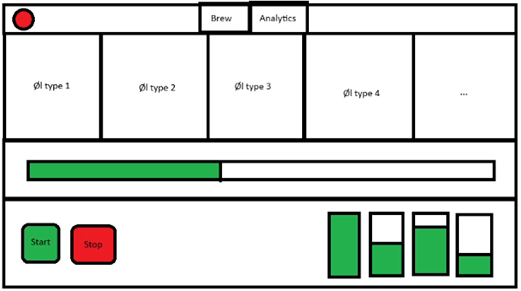
\includegraphics[width=1\textwidth]{img/frontend-draft.png}
      \caption{Early draft of the user interface}
      \label{fig:Frontend_draft}
  \end{figure}
\end{center}
With attention to the user experience, the UI was designed to be intuitive and easy to use, with a clear and simple layout and a minimalistic design. \newline
At the top of the page, the user should presented with 2 tabs: the \textit{Brew} tab and the \textit{Analytic} tab.  \newline
The \textit{Brew} tab is the default tab, and this is where the user can initiate the beer production process. \newline
The user is at the top presented with a column of the available beer types, and the user can select the desired beer type by clicking on the corresponding button. \newline
Below the beer type buttons a progress bar is displayed, this progress bar will be updated to reflect the current stage of the beer production process. \newline
At the bottom of the page, the column is divided into 2 sections: the left section contains \textit{Control buttons} to either start or stop the production, and the right side contains the \textit{Silo fill level} which visually indicates the current level of material stored in the silo. \newline
To brew a beer, the user simply selects the desired beer type, followed by pressing the big green \textit{Start} button at the bottom left.
The \textit{Analytic} tab is where the user should be view the data collected from the beer production process in a simple column-based view. Such as: temperature, vibration, maintenance status, completed batches and failed batches. \newline

\subsection{Backend}
The backend component of the beer production system should be implemented using Node.js, a versatile JavaScript runtime known for its efficiency in building scalable and high-performance server-side applications. Leveraging the strengths of Node.js, we aim to create a secure and reliable back-end that seamlessly communicates with the front end and the PLC-controlled beer production machine.
Node was chosen over Milo, for various reasons. Some of the thoughts behind the reasoning include:
\begin{itemize}
  \item Node is a more popular framework, which means it has a larger community, and is more well-documented, which makes it easier to find solutions to problems.  
  \item The framework is more versatile compared to Milo, which allows for more flexibility in terms of both development and time spent developing. 
  \item Lastly, it runs on the newest version of Java, which means that it is more likely to be supported in the future and is less likely to be affected by potential flaws from the previous versions of Java. \newline
\end{itemize}
This choice of using Node also enabled us to implement and use the OPC-UA library, which allowed us to easily implement a secure communication with the beer machine by automatically generating the certificate needed for the communication between the systems.

\subsubsection{Communication}
The backend should be responsible for handling routing and requests for communication within the system, aswell as the dataprocessing to fully automate different processes such as brewing and maintenance. This should be implemented using a RESTful API, in form of different endpoints with different responsibles. \newline 
The backend should be able to \textit{GET} the state of the beer machine, and its inventory. This is needed to handle the beer procressing and the maintenance process within the backend.\newline
Furthermore, the backend should be able to \textit{POST} a beer order to the beer machine into production. This is needed to handle the beer production process.\newline
Lastly, the backend should be able to \textit{GET} the data collected from the beer production process and \textit{POST} the data to the database. This is needed to handle the data processing and logging of the beer production process.
The design choice of using a RESTful API, allows for a clear separation of concerns, as each endpoint is responsible for a specific task, which in turn allows for a more efficient development process, as each endpoint and its logic can be developed and tested individually.

\subsection{Simulation}
Incorporating the provided ARsim simulation tool early on into our development process should be at high priority for this project to reduce development time in terms of testing. 
The early integration will allow us to speed up the development time from the very beginning, as most of our program's functionalities then can be tested directly without the need for direct access to the physical machine.
The tool allows us to interact with ARsim in a manner similar to how our software would communicate with the actual machine, and also enable concurrent tests of multiple different things without interfering with one another.


\subsubsection{ARsim Integration}
The early ARsim simulation tool integration into the development process, to mimic the behavior of the beer machine will allow us to speed up the development time from the very start of the project, as most of our program's functionalities could be tested thoroughly without the need of the physical beer machine.
This integration will also allow us to interact with ARsim in a manner similar to how our software would communicate with the actual hardware, and enabled multiple people to test multiple different things without interfering with one another. 

\subsection{Summary}
We chose to design our project using the client-server model, as it allows for a clear separation of concerns and enables us to have a more efficient development process, as each component can be developed and tested individually. \newline
This architecture separates the system into three deployments: The web service, the database service, and the physical beer machine. \newline
The web service consists of the frontend, the backend and the OPC Client. The frontend is developed using React, and the backend is developed using Node to meet our requirements. The use of JavaScript for both the frontend and the backend, allows for a more efficient development process, as the same language can be used for both components. \newline
The communication between the frontend, the backend and the beer machine is implemented using a RESTful API, where every endpoint has a specific responsibilit to ensure a clear separation of concerns. \newline
Lastly, the ARsim simulation tool should be integrated early into the development process to mimic the behavior of the beer machine and allow for a more efficient development process. 